\chapter{Data Sources}\label{Chp:ref:data sources}

At the source of every inversion is data in the form of gravity anomaly or
magnetic flux density values for at least a part of the region of interest.
These usually come from surveys and are preprocessed to correct for various
factors and distortions.
This chapter provides an overview of the classes related to data input for
inversions.

\section{General Interface}
The inversion module comes with a number of classes that can read gridded
(raster) data on a 2-dimensional plane from file or provide artificial values
for testing purposes. These classes all derive from the abstract
\class{DataSource} class and override methods that return information about
the data and the values themselves.
The \class{DomainBuilder} class is responsible for creating an \escript domain
with a suitable grid spacing and spatial extents that include all data sources
attached to it (see Figure~\ref{fig:domainBuilder}).
%
\begin{figure}[ht]
    \centering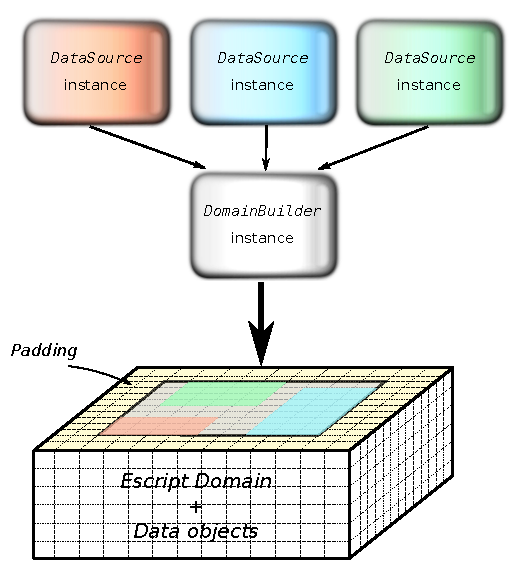
\includegraphics{domainbuilder}
    \caption{\class{DataSource} instances are added to a \class{DomainBuilder}
        which creates a suitable domain and \Data objects for the inversion}
    \label{fig:domainBuilder}
\end{figure}
%
Notice that in the figure there are cells in the region of interest that are
not covered by any data source instance.
Ideally, all data sources used for an inversion have the same spatial resolution
and are spatially adjacent so that all cells have a value but this is not a
requirement.


\section{Domain Builder}\label{Chp:ref:domain builder}
Every inversion requires one \class{DomainBuilder} instance which has the
following methods:

\begin{classdesc}{DomainBuilder}{\optional{dim=3}}
Constructor for the domain builder. \member{dim} sets the dimensionality of the
target domain and must be 2 or 3. By default a 3-dimensional domain is created.
\end{classdesc}

\begin{methoddesc}[DomainBuilder]{addSource}{source}
    Adds survey data \member{source} (a \class{DataSource} object) to the domain
    builder. The dimensionality of the data must be less than or equal to the
    domain dimensionality.
\end{methoddesc}

\begin{methoddesc}[DomainBuilder]{getDomain}{}
returns the \escript domain of the inversion, see~\cite{ESCRIPT}.
\end{methoddesc}

\section{ER Mapper Raster Data}

\section{NetCDF Data}
An example script how to create a data input file for both gravity and magnetic data using the NetCDF file format~\cite{netcdf}
is available in the script \examplefile{create_ncinput.py}. To plot an input file using matplotlib~\cite{matplotlib} 
is avilable in the script \examplefile{show_ncinput.py}.

\section{Synthetic Data}

